% Do not forget to include Introduction
%---------------------------------------------------------------
% \chapter{Introduction}
% uncomment the following line to create an unnumbered chapter
\chapter*{Introduction}\addcontentsline{toc}{chapter}{I: Introduction}\markboth{Introduction}{Introduction}
%---------------------------------------------------------------
\setcounter{page}{1}

% The following environment can be used as a mini-introduction for a chapter. Use that any way it pleases you (or comment it out). It can contain, for instance, a summary of the chapter. Or, there can be a quotation.
\begin{chapterabstract}
	\lipsum[1]
\end{chapterabstract}

A survey of the American National Highway Traffic Safety Administration (NHTSA) reports that nearly 94\% of road accidents are due to human errors [1]. 
These human-related mistakes are mainly classified as driver distraction, drunk or otherwise impaired driving, lack of attention, violation of the traffic rules, limited view of traffic conditions, and jay-walking pedestrians [2]. 
The lack of rule obedience, the increasing number of vehicles on roads, and improper road culture have therefore motivated officials, manufacturers, and legislators to make substantial improvements in transportation systems. 
There are growing research and development attempts to enhance safety and automation capability of autonomous vehicles (AVs), prevent traffic accidents, and create a better road infrastructure. 
The potential benefits of AVs are improved convenience, operational safety (especially for seniors and people with reduced mobility) [3], reduced CO2 emissions [4], diminished transportation costs [5], improved safety [6, 7], and reduced traffic density [8].

%---------------------------------------------------------------
\section{Motivation}
%---------------------------------------------------------------

%---------------------------------------------------------------
\section{Problem Statement \& Objectives}
%---------------------------------------------------------------

%---------------------------------------------------------------
\section{Delimitations}
%---------------------------------------------------------------

%---------------------------------------------------------------
\section{Research Questions \& Methodology}
%---------------------------------------------------------------

%---------------------------------------------------------------
\section{Thesis Outline}
%---------------------------------------------------------------


%%%%%%%%%%%%%%%%%%%%%%%%%%%%%%%%%%%%%%%%%%%%%%%%%%%%%%%%%%%%%%%%


\chapter{II: ADRIANA (Preliminaries)}\addcontentsline{toc}{chapter}{II: ADRIANA}\markboth{II: ADRIANA}{II: ADRIANA}
%---------------------------------------------------------------

% The following environment can be used as a mini-introduction for a chapter. Use that any way it pleases you (or comment it out). It can contain, for instance, a summary of the chapter. Or, there can be a quotation.
\begin{chapterabstract}
	\lipsum[1]
\end{chapterabstract}

This chapter provides a theoretical background required for understanding of the thesis' problematics and accomplishing the tasks set.
It contains a general overview of the current state of driving automation, including a detailed taxonomy and comparison of the various levels of automation.
It is important to specify, that the focus is being made mainly on the very \textit{taxonomy} without going into the details of processes, interactions of conditional constituents \& techologies coherent with each level individually.

Later, the analysis of mechanisms that make the driving automation possible (inter-ECUs communication) is being done, exploring the various communication protocols and standards.
The focus is being made on possibilities of data manipulation \& security issues that might be useful in the terms of pending implementation of the system for signals manipulation on the Automotive Ethernet.

%---------------------------------------------------------------
\section{Taxonomy of Driving Automation}
%---------------------------------------------------------------
In order to dive into the topic of driving automation, the \textit{driving} itsef should be overviewed at first.

Driving entails a variety of decisions and actions, which may or may not involve a vehicle being in motion, or even being in an active lane of traffic. 
The overall act of driving can be divided into three types of driver effort: strategic, tactical, and operational (Michon, 1985).

\textit{Strategic} effort involves trip planning, such as deciding whether, when and where to go, how to travel, best routes to take, etc.

\textit{Tactical} effort involves maneuvering the vehicle in traffic during a trip, including deciding whether and when to overtake another vehicle or change lanes, selecting an appropriate speed, checking mirrors, etc.

\textit{Operational} effort involves split-second reactions that can be considered pre-cognitive or innate, such as making-micro-corrections to steering, braking and accelerating to maintain lane position in traffic or to avoid a sudden obstacle or hazardous event in the vehicle’s pathway.

The schematic view of the driving task can be seen in Figure \ref{fig:driving_task}.

\begin{figure}[h]
  \centering
  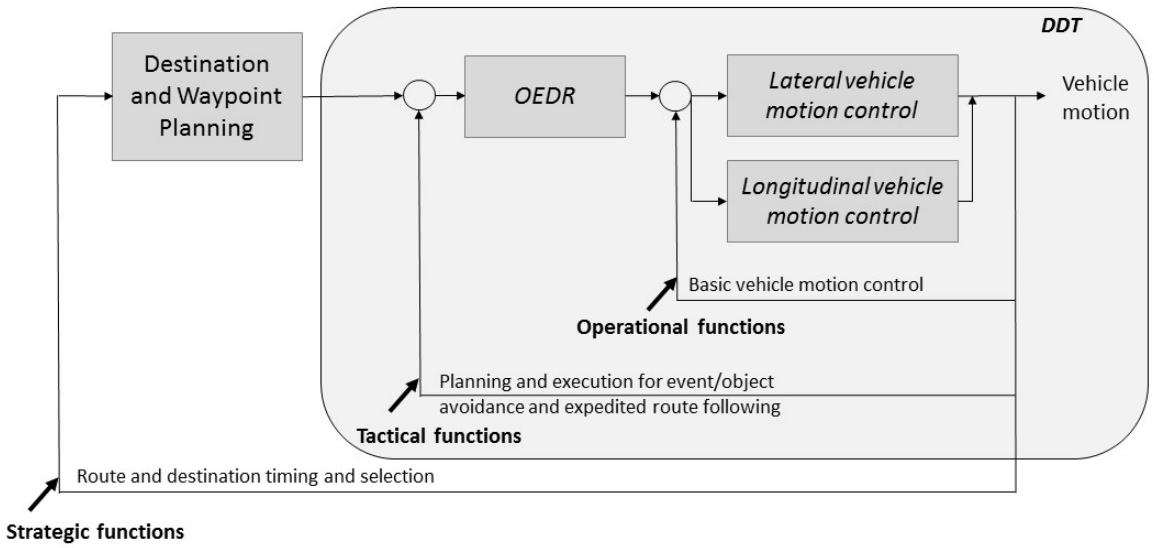
\includegraphics[width=0.9\textwidth]{images/ddt_explained.PNG}
  \caption{Schematic (not a control diagram) view of the driving task.}
  \label{fig:driving_task}
\end{figure}

A self-driving car, also known as an \textit{autonomous car}, is a car that is capable of traveling without human input \cite{Xie}.
Self-driving cars use sensors to perceive their surroundings, such as optical and thermographic cameras, radar, lidar, ultrasound/sonar, GPS, odometry and inertial measurement units \cite{Xie2}.
Also, further technologies used to achieve autonomous driving might include several forms of artificial intelligence \cite{atakishiyev2023explainable}.

Researchers \boldorange{forecast} that by 2025 approximately 8 million autonomous or semi-autonomous vehicles will be used on the road.
Before merging onto roadways, self-driving cars will first have to progress through several levels of driver assistance technology advancements.

SAE J3016 defines 6 levels of automation, sketching an incremental evolution from no automation to fully autonomous vehicles \cite{Serban2020}. 
Central to this taxonomy are the respective roles of the (human) \textit{user} and the \textit{driving automation system} (DAS) in relation to each other.
Since changes in the functionality of a \textit{driving automation system} change the role of the (human) \textit{user}, they provide a basis for categorizing such system \textit{features}. 
For example:

% TODO: make word italic according to the document
\begin{itemize}

  \item If the driving automation system performs the sustained longitudinal and/or lateral vehicle motion control subtasks of the DDT
  \footnote{
      All of the real-time operational and tactical functions required to operate a vehicle in on-road traffic, excluding the strategic functions such as trip scheduling and selection of destinations and waypoints, and including, without limitation, the following subtasks:
      \begin{enumerate}
        \item Lateral vehicle motion control via steering (operational).
        \item Longitudinal vehicle motion control via acceleration and deceleration (operational).
        \item Monitoring the driving environment via object and event detection, recognition, classification, and response preparation (operational and tactical).
        \item Object and event response execution (operational and tactical).
        \item Maneuver planning (tactical).
        \item Enhancing conspicuity via lighting, sounding the horn, signaling, gesturing, etc. (tactical)
      \end{enumerate}
  }, the driver does not do so, although s/he is expected to complete the DDT. 
  This division of roles corresponds to Levels 1 and 2.
  \item If the driving automation system performs the entire DDT, the user does not do so. However, if a DDT fallback-ready user is expected to take over the DDT when a DDT performance-relevant system failure occurs or when the driving automation system is about to leave its operational design domain (ODD)\footnote{Specified by manufacturer.}, then that user is expected to be receptive and able to resume DDT performance when alerted to the need to do so. 
  This division of roles corresponds to Level 3.
  \item Lastly, if a driving automation system can perform the entire DDT and DDT fallback either within a prescribed ODD (Level 4) or in all driver-manageable on-road operating situations (Level 5) then any users present in the vehicle while the ADS is engaged are passengers. 
  
\end{itemize}

Although the vehicle fulfills a role in this driving automation taxonomy, it does not change the role of the user in performing the DDT. 
By contrast the role played by the driving automation system complements the role of the user in performing the DDT, and in that sense changes it.

In this way, driving automation systems are categorized into levels based on:

\begin{enumerate}

  \item Whether the driving automation system performs either the longitudinal or the lateral vehicle motion control subtask of the DDT.
  \item Whether the driving automation system performs both the longitudinal and the lateral vehicle motion control subtasks of the DDT simultaneously.
  \item Whether the driving automation system also performs the OEDR subtask of the DDT.
  \item Whether the driving automation system also performs DDT fallback.
  \item Whether the driving automation system is limited by an ODD. 

\end{enumerate}

Table 1 summarizes the six levels of driving automation in terms of these five elements.
It is worth mentioning, that SAE’s levels of driving automation are descriptive and informative, rather than normative, and technical rather than legal.
Elements indicate minimum rather than maximum capabilities for each level \cite{saej3016}.

\begin{table}[]
  \centering
  \catcode`\-=12 %%!!!!!!!!!!!!!!!!!!!!!!!!!!!!!!!!!!!!!!!!!!!!!!!!!!!!

\begin{adjustbox}{width=\textwidth} % fill to the whole page

  \begin{tabular}{|lcllcccc|}
    \hline
    \multicolumn{1}{|l|}{\multirow{2}{*}{}}                                                     & \multicolumn{1}{c|}{\multirow{2}{*}{\rotatebox[origin=c]{90}{\textbf{Level} \;}}} & \multicolumn{1}{c|}{\multirow{2}{*}{\textbf{Name}}}                                                      & \multicolumn{1}{c|}{\multirow{2}{*}{\textbf{Narrative Definition}}}                                                                                                                                                                                                                                                                                                          & \multicolumn{2}{c|}{\textbf{DDT}}                                                                                                                                                   & \multicolumn{1}{c|}{\multirow{2}{*}{\textbf{\begin{tabular}[c]{@{}c@{}}DDT \\ Fallback\end{tabular}}}}                                 & \multirow{2}{*}{\textbf{ODD}} \\ \cline{5-6}
    \multicolumn{1}{|l|}{}                                                                      & \multicolumn{1}{c|}{}                                                             & \multicolumn{1}{c|}{}                                                                                    & \multicolumn{1}{c|}{}                                                                                                                                                                                                                                                                                                                                                        & \multicolumn{1}{l|}{\textbf{\begin{tabular}[c]{@{}l@{}}Sustained\\ Lateral and \\ Longitudinal \\ Vechicle \\ Motion \\ Control\end{tabular}}} & \multicolumn{1}{l|}{\textbf{OEDR}} & \multicolumn{1}{c|}{}                                                                                                                  &                               \\ \hline
    \multicolumn{8}{|c|}{\textbf{Driver Performs Part or All of the DDT}}                                                                                                                                                                                                                                                                                                                                                                                                                                                                                                                                                                                                                                                                                                                                                                                                                                                                                                             \\ \hline
    \multicolumn{1}{|l|}{}                                                                      & \multicolumn{1}{c|}{\textbf{0}}                                                   & \multicolumn{1}{l|}{\textit{\begin{tabular}[c]{@{}l@{}}No Driving\\ Automation\end{tabular}}}            & \multicolumn{1}{l|}{\begin{tabular}[c]{@{}l@{}}The performance by the driver\\ of the entire DDT, even when\\ enchaned by ASSs.\end{tabular}}                                                                                                                                                                                                                                & \multicolumn{1}{c|}{Driver}                                                                                                                    & \multicolumn{1}{c|}{Driver}        & \multicolumn{1}{c|}{Driver}                                                                                                            & n/a                           \\ \hline
    \multicolumn{1}{|l|}{\multirow{2}{*}{\rotatebox[origin=c]{90}{\textbf{Driver Support}}}}    & \multicolumn{1}{c|}{\textbf{1}}                                                   & \multicolumn{1}{l|}{\textit{\begin{tabular}[c]{@{}l@{}}Driver\\ Assistance\end{tabular}}}                & \multicolumn{1}{l|}{\begin{tabular}[c]{@{}l@{}}The sustained and ODD-specific\\ execution by a DAS of either the\\ lateral or longitudinal vehicle\\ motion control subtask of the DDT\\ (but not both simultaneously) with\\ the expectation that the driver\\ performs the remainder of the DDT.\end{tabular}}                                                             & \multicolumn{1}{c|}{\begin{tabular}[c]{@{}c@{}}Driver\\ and\\ System\end{tabular}}                                                             & \multicolumn{1}{c|}{Driver}        & \multicolumn{1}{c|}{Driver}                                                                                                            & Limited                       \\ \cline{2-8} 
    \multicolumn{1}{|l|}{}                                                                      & \multicolumn{1}{c|}{\textbf{2}}                                                   & \multicolumn{1}{l|}{\textit{\begin{tabular}[c]{@{}l@{}}Partial\\ Driving\\ Automation\end{tabular}}}     & \multicolumn{1}{l|}{\begin{tabular}[c]{@{}l@{}}The sustained and ODD-specific\\ execution by a DAS of both the\\ lateral and longitudinal vehicle\\ motion control subtasks of the DDT\\ with the expectation that the driver\\ completes the OEDR subtask and\\ supervises the DAS.\end{tabular}}                                                                           & \multicolumn{1}{c|}{System}                                                                                                                    & \multicolumn{1}{c|}{Driver}        & \multicolumn{1}{c|}{Driver}                                                                                                            & Limited                       \\ \hline
    \multicolumn{8}{|c|}{\textbf{ADS Performs the Entire DDT (While Enabled)}}                                                                                                                                                                                                                                                                                                                                                                                                                                                                                                                                                                                                                                                                                                                                                                                                                                                                                                        \\ \hline
    \multicolumn{1}{|l|}{\multirow{3}{*}{\rotatebox[origin=c]{90}{\textbf{Automated Driving}}}} & \multicolumn{1}{c|}{\textbf{3}}                                                   & \multicolumn{1}{l|}{\textit{\begin{tabular}[c]{@{}l@{}}Conditional\\ Driving\\ Automation\end{tabular}}} & \multicolumn{1}{l|}{\begin{tabular}[c]{@{}l@{}}The sustained and ODD-specific\\ performance by an ADS of the\\ entire DDT with the expectation\\ that the DDT fallback-ready user\\ is receptive to ADS-issued requests\\ to intervene, as well as to DDT\\ performance-relevant system\\ failures in other vehicle systems,\\ and will respond appropriately.\end{tabular}} & \multicolumn{1}{c|}{System}                                                                                                                    & \multicolumn{1}{c|}{System}        & \multicolumn{1}{c|}{\begin{tabular}[c]{@{}c@{}}Fallback-\\ Ready\\ User\\ (becomes\\ the driver\\ during the\\ fallback)\end{tabular}} & Limited                       \\ \cline{2-8} 
    \multicolumn{1}{|l|}{}                                                                      & \multicolumn{1}{c|}{\textbf{4}}                                                   & \multicolumn{1}{l|}{\textit{\begin{tabular}[c]{@{}l@{}}High\\ Driving\\ Automation\end{tabular}}}        & \multicolumn{1}{l|}{\begin{tabular}[c]{@{}l@{}}The sustained and ODD-specific\\ performance by an ADS of the\\ entire DDT and DDT fallback\\ without any expectation that a user\\ will need to intervene.\end{tabular}}                                                                                                                                                     & \multicolumn{1}{c|}{System}                                                                                                                    & \multicolumn{1}{c|}{System}        & \multicolumn{1}{c|}{System}                                                                                                            & Limited                       \\ \cline{2-8} 
    \multicolumn{1}{|l|}{}                                                                      & \multicolumn{1}{c|}{\textbf{5}}                                                   & \multicolumn{1}{l|}{\textit{\begin{tabular}[c]{@{}l@{}}Full\\ Driving\\ Automation\end{tabular}}}        & \multicolumn{1}{l|}{\begin{tabular}[c]{@{}l@{}}The sustained and unconditional\\ (i.e., not ODD-specific)\\ performance by an ADS of the\\ entire DDT and DDT fallback\\ wothout any expectation that a user\\ will need to intervene.\end{tabular}}                                                                                                                         & \multicolumn{1}{c|}{System}                                                                                                                    & \multicolumn{1}{c|}{System}        & \multicolumn{1}{c|}{System}                                                                                                            & Unlimited*                    \\ \hline
  \end{tabular}

\end{adjustbox}
  \vspace{0.35cm}
  \caption{Summary of levels of driving automation according to SAE J3016.}
  \label{tab:SAEJ3016}
\end{table}

In this table, “system” refers to the driving automation system or ADS, as appropriate.
Definitions of some terms that seem to be obvious ("driver", for instacne) are omitted for the sake of brevity.
In addition, as it was implicitly mentioned earlier, the DDT does not include strategic aspects of the driving task, such as determining destination(s) and deciding when to travel.

\begin{note}
  \textit{“Unconditional/not ODD-specific”} means that the ADS can operate the vehicle on-road anywhere within its region of the world and under all road conditions in which a conventional vehicle can be reasonably operated by a typically skilled human driver. 
  This means, for example, that there are no design-based weather, time-of-day, or-geographical restrictions on where and when the ADS can operate the vehicle. 
  However, there may be conditions not manageable by a driver in which the ADS would also be unable to complete a given trip (e.g., white-out snow storm, flooded roads, glare ice, etc.) until or unless the adverse conditions clear. 
  At the onset of such unmanageable conditions the ADS would perform the DDT fallback to achieve a minimal risk condition (e.g., by pulling over to the side of the road and waiting for the conditions to change). 
\end{note}

Figure \ref{fig:driving_task} illustrates how a trip could be completed by use of various combinations of driving automation features engaged at different levels of driving automation.

\begin{figure}[!ht]
	\centering
	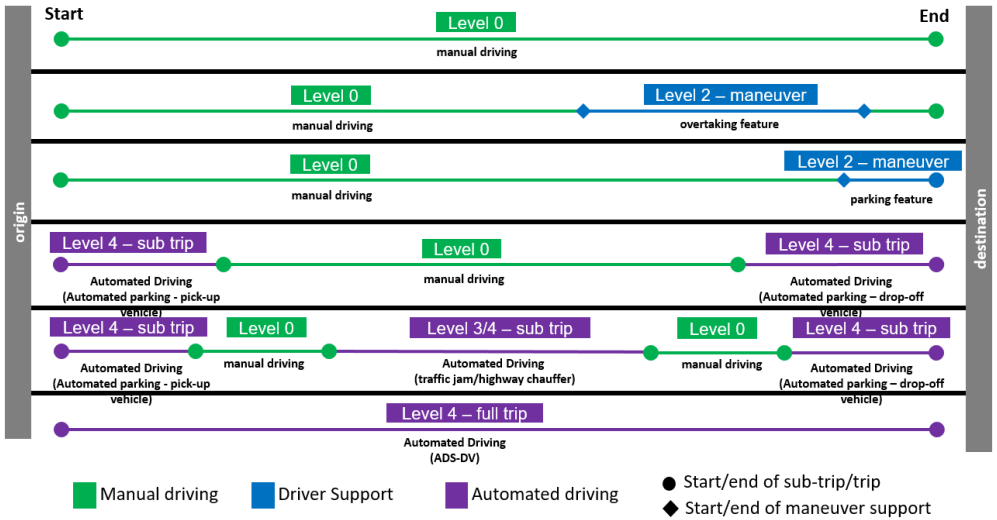
\includegraphics[width=0.9\textwidth]{images/driving_automation.PNG}
	\caption{Examples of driving automation system features/types that could be available during a given trip.}
  \label{img:driving_automation}
\end{figure}

\begin{figure}[h]
  \centering
  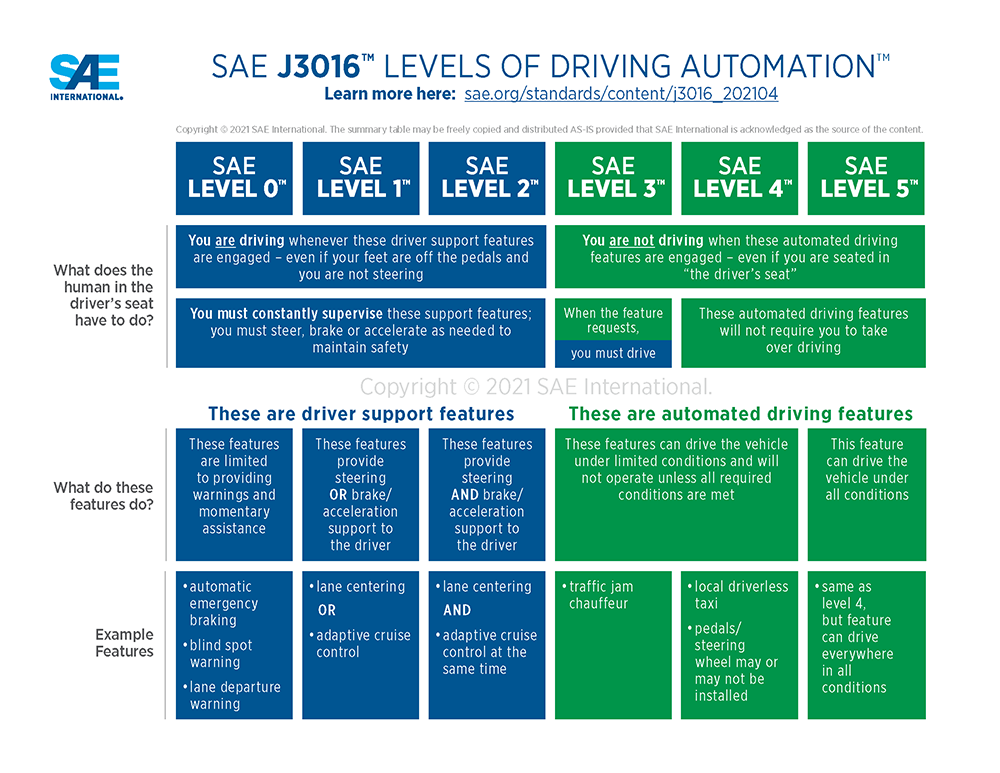
\includegraphics[width=0.9\textwidth]{images/sae-j3016-chart.png}
  \caption{SAE J3016}
  \label{fig:SAEJ3016}
\end{figure}

%---------------------------------------------------------------
\section{Internal Networks}
%---------------------------------------------------------------

%---------------------------------------------------------------
\section{Controller Area Network (CAN)}
%---------------------------------------------------------------

%---------------------------------------------------------------
\subsection{J1939}
%---------------------------------------------------------------

%---------------------------------------------------------------
\subsection{OBD2}
%---------------------------------------------------------------

%---------------------------------------------------------------
\subsection{LIN (Local Interconnect Network)}
%---------------------------------------------------------------

%---------------------------------------------------------------
\subsection{UDS (Unified Diagnostic Services)}
%---------------------------------------------------------------

%---------------------------------------------------------------
\section{CAN Bus Errors}
%---------------------------------------------------------------

%---------------------------------------------------------------
\section{Data Manipulation \& Security}
%---------------------------------------------------------------

%%%%%%%%%%%%%%%%%%%%%%%%%%%%%%%%%%%%%%%%%%%%%%%%%%%%%%%%%%%%%%%%





%%%%%%%%%%%%%%%%%%%%%%%%%%%%%%%%%%%%%%%%%%%%%%%%%%%%%%%%%%%%%%%%


\chapter{III: BEATRIX (Testing System Requirements)}\addcontentsline{toc}{chapter}{III: BEATRIX}\markboth{III: BEATRIX}{III: BEATRIX}
%---------------------------------------------------------------

% The following environment can be used as a mini-introduction for a chapter. Use that any way it pleases you (or comment it out). It can contain, for instance, a summary of the chapter. Or, there can be a quotation.
\begin{chapterabstract}
	\lipsum[1]
\end{chapterabstract}

\lipsum[2][1-4]{} [1]

\lipsum[4]

%---------------------------------------------------------------
\section{Software Requirements}
%---------------------------------------------------------------

%---------------------------------------------------------------
\section{Hardware Requirements}
%---------------------------------------------------------------


%%%%%%%%%%%%%%%%%%%%%%%%%%%%%%%%%%%%%%%%%%%%%%%%%%%%%%%%%%%%%%%%





%%%%%%%%%%%%%%%%%%%%%%%%%%%%%%%%%%%%%%%%%%%%%%%%%%%%%%%%%%%%%%%%


\chapter{IV: CALEDONIA}\addcontentsline{toc}{chapter}{IV: CALEDONIA}\markboth{IV: CALEDONIA}{IV: CALEDONIA}
%---------------------------------------------------------------

% The following environment can be used as a mini-introduction for a chapter. Use that any way it pleases you (or comment it out). It can contain, for instance, a summary of the chapter. Or, there can be a quotation.
\begin{chapterabstract}
	\lipsum[1]
\end{chapterabstract}

\lipsum[2][1-4]{} [1]

\lipsum[4]

%---------------------------------------------------------------
\section{Ut enim ad minim veniam}
%---------------------------------------------------------------


%%%%%%%%%%%%%%%%%%%%%%%%%%%%%%%%%%%%%%%%%%%%%%%%%%%%%%%%%%%%%%%%





%%%%%%%%%%%%%%%%%%%%%%%%%%%%%%%%%%%%%%%%%%%%%%%%%%%%%%%%%%%%%%%%


\chapter{V: DELORES}\addcontentsline{toc}{chapter}{V: DELORES}\markboth{V: DELORES}{V: DELORES}
%---------------------------------------------------------------

% The following environment can be used as a mini-introduction for a chapter. Use that any way it pleases you (or comment it out). It can contain, for instance, a summary of the chapter. Or, there can be a quotation.
\begin{chapterabstract}
	\lipsum[1]
\end{chapterabstract}

\lipsum[2][1-4]{} [1]

\lipsum[4]

%---------------------------------------------------------------
\section{Ut enim ad minim veniam}
%---------------------------------------------------------------


%%%%%%%%%%%%%%%%%%%%%%%%%%%%%%%%%%%%%%%%%%%%%%%%%%%%%%%%%%%%%%%%





%%%%%%%%%%%%%%%%%%%%%%%%%%%%%%%%%%%%%%%%%%%%%%%%%%%%%%%%%%%%%%%%


\chapter{VI: RESULTS}\addcontentsline{toc}{chapter}{VI: RESULTS}\markboth{VI: RESULTS}{VI: RESULTS}
%---------------------------------------------------------------

% The following environment can be used as a mini-introduction for a chapter. Use that any way it pleases you (or comment it out). It can contain, for instance, a summary of the chapter. Or, there can be a quotation.
\begin{chapterabstract}
	\lipsum[1]
\end{chapterabstract}

\lipsum[2][1-4]{} [1]

\lipsum[4]

%---------------------------------------------------------------
\section{Ut enim ad minim veniam}
%---------------------------------------------------------------


%%%%%%%%%%%%%%%%%%%%%%%%%%%%%%%%%%%%%%%%%%%%%%%%%%%%%%%%%%%%%%%%










\lipsum[6-7]

\begin{figure}
\centering
%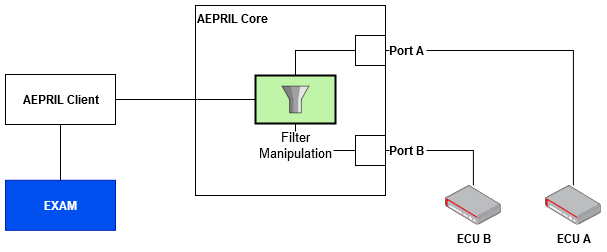
\includegraphics[scale=0.4]{pic/index}
\resizebox{\textwidth}{!}{
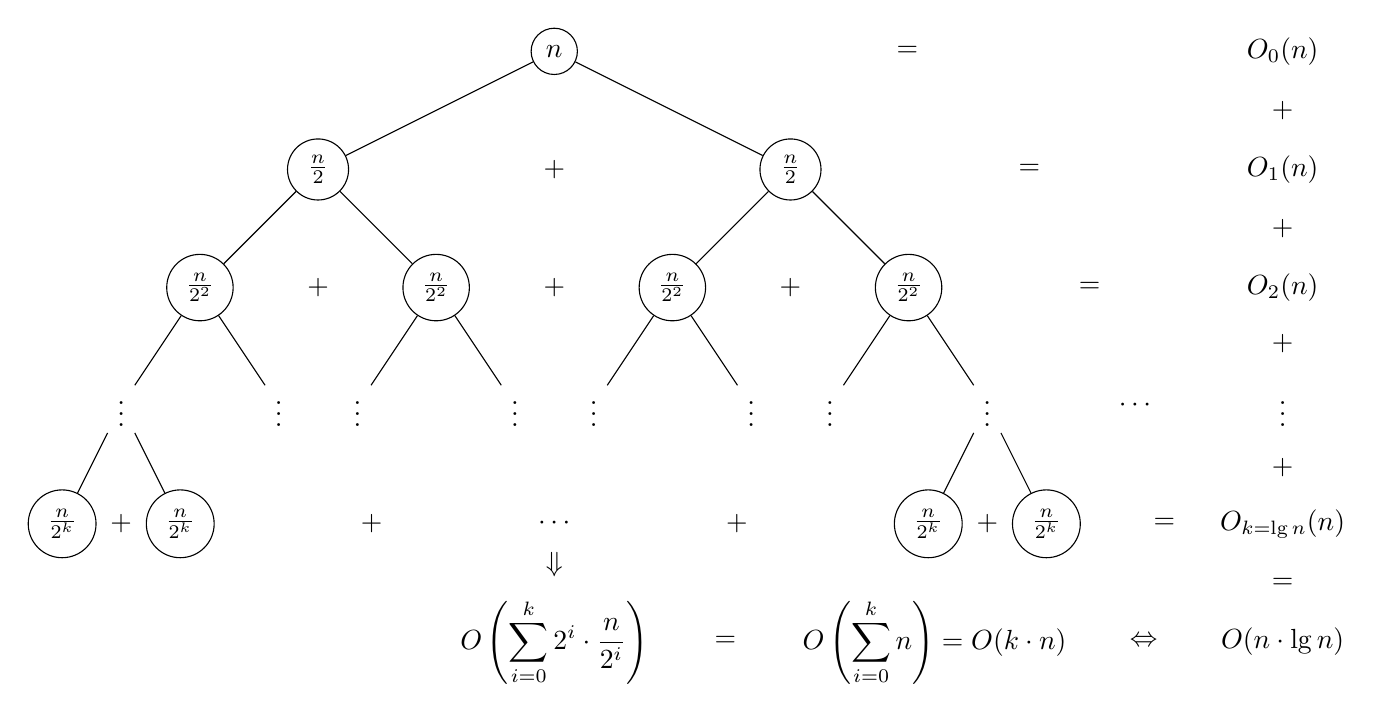
\begin{tikzpicture}[level/.style={sibling distance=60mm/#1}]
\node [circle,draw] (z){$n$}
  child {node [circle,draw] (a) {$\frac{n}{2}$}
    child {node [circle,draw] (b) {$\frac{n}{2^2}$}
      child {node {$\vdots$}
        child {node [circle,draw] (d) {$\frac{n}{2^k}$}}
        child {node [circle,draw] (e) {$\frac{n}{2^k}$}}
      } 
      child {node {$\vdots$}}
    }
    child {node [circle,draw] (g) {$\frac{n}{2^2}$}
      child {node {$\vdots$}}
      child {node {$\vdots$}}
    }
  }
  child {node [circle,draw] (j) {$\frac{n}{2}$}
    child {node [circle,draw] (k) {$\frac{n}{2^2}$}
      child {node {$\vdots$}}
      child {node {$\vdots$}}
    }
  child {node [circle,draw] (l) {$\frac{n}{2^2}$}
    child {node {$\vdots$}}
    child {node (c){$\vdots$}
      child {node [circle,draw] (o) {$\frac{n}{2^k}$}}
      child {node [circle,draw] (p) {$\frac{n}{2^k}$}
        child [grow=right] {node (q) {$=$} edge from parent[draw=none]
          child [grow=right] {node (q) {$O_{k = \lg n}(n)$} edge from parent[draw=none]
            child [grow=up] {node (r) {$\vdots$} edge from parent[draw=none]
              child [grow=up] {node (s) {$O_2(n)$} edge from parent[draw=none]
                child [grow=up] {node (t) {$O_1(n)$} edge from parent[draw=none]
                  child [grow=up] {node (u) {$O_0(n)$} edge from parent[draw=none]}
                }
              }
            }
            child [grow=down] {node (v) {$O(n \cdot \lg n)$}edge from parent[draw=none]}
          }
        }
      }
    }
  }
};
\path (a) -- (j) node [midway] {+};
\path (b) -- (g) node [midway] {+};
\path (k) -- (l) node [midway] {+};
\path (k) -- (g) node [midway] {+};
\path (d) -- (e) node [midway] {+};
\path (o) -- (p) node [midway] {+};
\path (o) -- (e) node (x) [midway] {$\cdots$}
  child [grow=down] {
    node (y) {$O\left(\displaystyle\sum_{i = 0}^k 2^i \cdot \frac{n}{2^i}\right)$}
    edge from parent[draw=none]
  };
\path (q) -- (r) node [midway] {+};
\path (s) -- (r) node [midway] {+};
\path (s) -- (t) node [midway] {+};
\path (s) -- (l) node [midway] {=};
\path (t) -- (u) node [midway] {+};
\path (z) -- (u) node [midway] {=};
\path (j) -- (t) node [midway] {=};
\path (y) -- (x) node [midway] {$\Downarrow$};
\path (v) -- (y)
  node (w) [midway] {$O\left(\displaystyle\sum_{i = 0}^k n\right) = O(k \cdot n)$};
\path (q) -- (v) node [midway] {=};
\path (e) -- (x) node [midway] {+};
\path (o) -- (x) node [midway] {+};
\path (y) -- (w) node [midway] {$=$};
\path (v) -- (w) node [midway] {$\Leftrightarrow$};
\path (r) -- (c) node [midway] {$\cdots$};
\end{tikzpicture}}
\caption{~Lorem ipsum dolor sit amet}\label{img:index}
\end{figure}

%---------------------------------------------------------------
\section{Ut enim ad minim veniam}
%---------------------------------------------------------------

\lipsum[2-4]

%---------------------------------------------------------------
\subsection{Ut enim ad minim veniam}
%---------------------------------------------------------------

Curabitur ligula sapien, pulvinar a vestibulum quis, facilisis vel sapien. Duis condimentum augue id magna semper rutrum. Aliquam ornare wisi eu metus. Fusce aliquam vestibulum ipsum. Vivamus ac leo pretium faucibus\ref{img:index}.

\begin{itemize}
    \item Ut enim ad minim veniam, quis nostrud
    \item Ut enim ad minim 
    \item Ut enim ad minim veniam, quis 
    \begin{itemize}
        \item Ut enim ad
        \item Ut enim ad
        \begin{itemize}
            \item Ut enim 
            \item Ut enim 
            \begin{itemize}
            \item Ut enim 
            \item Ut enim 
        \end{itemize}
        \end{itemize}
    \end{itemize}
\end{itemize}

\section{Class aptent taciti}

\lipsum[2]

\subsection{Class aptent taciti}

\lipsum[6-7]

\begin{enumerate}
    \item Ut enim ad minim veniam, quis nostrud
    \item Ut enim ad minim 
    \item Ut enim ad minim veniam, quis 
    \begin{enumerate}
        \item Ut enim ad
        \item Ut enim ad
        \begin{enumerate}
            \item Ut enim 
            \item Ut enim 
            \begin{enumerate}
            \item Ut enim 
            \item Ut enim 
        \end{enumerate}
        \end{enumerate}
    \end{enumerate}
\end{enumerate}


%---------------------------------------------------------------
\section{Ut enim ad minim veniam, quis nostrud}
%---------------------------------------------------------------

Ut enim ad minim veniam, quis nostrud exercitation ullamco laboris nisi ut aliquip ex ea commodo consequat. Nulla non arcu lacinia neque faucibus fringilla. Vestibulum erat nulla, ullamcorper nec, rutrum non, nonummy ac, erat. Aliquam erat volutpat. Proin pede metus, vulputate nec, fermentum fringilla, vehicula vitae, justo.\footnote{Ut enim ad minim veniam, quis nostrud exercitation.} Etiam dictum tincidunt diam. In laoreet, magna id viverra tincidunt, sem odio bibendum justo, vel imperdiet sapien wisi sed libero. Nulla est. Maecenas fermentum, sem in pharetra pellentesque, velit turpis volutpat ante, in pharetra metus odio a lectus. Duis aute irure dolor in reprehenderit in voluptate velit esse cillum dolore eu fugiat nulla pariatur. 

\begin{lstlisting}[caption={~Zbytečný kód},label=list:8-6,captionpos=t,float,abovecaptionskip=-\medskipamount,belowcaptionskip=\medskipamount,language=C]
    #include<stdio.h>
    #include<iostream>
    // A comment
    int main(void)
    {
        printf("Hello World\n");
        return 0;
    }
\end{lstlisting}

%%%%%%%%%%%%%%%%%%%%%%%%%%%%%%%%%
% alternative using package minted for source highlighting
% package minted requires execution with `-shell-escape'
% e.g., `xelatex -shell-escape ctufit-thesis.tex'
% \begin{listing}
% \caption{Zbytečný kód}\label{list:8-6}
% \begin{minted}{C}
%     #include<stdio.h>
%     #include<iostream>
%     // A comment
%     int main(void)
%     {
%         printf("Hello World\n");
%         return 0;
%     }
% \end{minted}
% \end{listing}
% %%%%%%%%%%%%%%%%%%%%%%%%%%%%%%%%%
Nullam feugiat, turpis at pulvinar vulputate, erat libero tristique tellus, nec bibendum odio risus sit amet ante. Aenean id metus id velit ullamcorper pulvinar. Fusce wisi. Integer lacinia. Aliquam id dolor. Pellentesque pretium lectus id turpis. Suspendisse sagittis ultrices augue. In laoreet, magna id viverra tincidunt, sem odio bibendum justo, vel imperdiet sapien wisi sed libero. Sed ac dolor sit amet purus malesuada congue. \cite{Crochemore2002}

Class aptent taciti sociosqu ad litora torquent per conubia nostra, per inceptos hymenaeos. Fusce suscipit libero eget elit. Etiam dui sem, fermentum vitae, sagittis id, malesuada in, quam. Aliquam id dolor. Curabitur bibendum justo non orci. Duis viverra diam non justo. Curabitur ligula sapien, pulvinar a vestibulum quis, facilisis vel sapien. Duis condimentum augue id magna semper rutrum. Aliquam ornare wisi eu metus. Fusce aliquam vestibulum ipsum. Vivamus ac leo pretium faucibus. \cite{Motwani2014}

%---------------------------------------------------------------
\subsection{Ut enim ad minim veniam, quis nostrud}
%---------------------------------------------------------------

Ut enim ad minim veniam, quis nostrud exercitation ullamco laboris nisi ut aliquip ex ea commodo consequat. Nulla non arcu lacinia neque faucibus fringilla. Vestibulum erat nulla, ullamcorper nec, rutrum non, nonummy ac, erat. Aliquam erat volutpat. Proin pede metus, vulputate nec, fermentum fringilla, vehicula vitae, justo. Etiam dictum tincidunt diam. In laoreet, magna id viverra tincidunt, sem odio bibendum justo. \cite{Sestakova2018} 

\begin{table}\centering
\caption[Příklad tabulky]{~Zadávání matematiky}\label{tab:matematika}
\begin{tabular}{l|l|c|c}
	Typ		& Prostředí		& \LaTeX{}ovská zkratka	& \TeX{}ovská zkratka	\tabularnewline \hline 
 	Text		& \verb|math|		& \verb|\(...\)|	& \verb|$...$|	\tabularnewline \hline
 	Displayed	& \verb|displaymath|	& \verb|\[...\]|	& \verb|$$...$$|	\tabularnewline 
\end{tabular}
\end{table}


Nulla est. Maecenas fermentum, sem in pharetra pellentesque, velit turpis volutpat ante, in pharetra metus odio a lectus. Duis aute irure dolor in reprehenderit in voluptate velit esse cillum dolore eu fugiat nulla pariatur. Nullam feugiat, turpis at pulvinar vulputate, erat libero tristique tellus, nec bibendum odio risus sit amet ante. Aenean id metus id velit ullamcorper pulvinar. 

\subsubsection{Class aptent taciti}

\begin{definition}[Optional label]
Class aptent taciti sociosqu ad litora torquent per conubia nostra, per inceptos hymenaeos. Fusce suscipit libero eget elit. Etiam dui sem, fermentum vitae, sagittis id, malesuada in, quam. Aliquam id dolor. Curabitur bibendum justo non orci.
\end{definition}

\begin{example}
Class aptent taciti sociosqu ad litora torquent per conubia nostra, per inceptos hymenaeos. Fusce suscipit libero eget elit. Etiam dui sem, fermentum vitae, sagittis id, malesuada in, quam. Aliquam id dolor. Curabitur bibendum justo non orci.
\end{example}

\begin{theorem}
Class aptent taciti sociosqu ad litora torquent per conubia nostra, per inceptos hymenaeos. Fusce suscipit libero eget elit. Etiam dui sem, fermentum vitae, sagittis id, malesuada in, quam. Aliquam id dolor. Curabitur bibendum justo non orci.
\end{theorem}

\begin{proof}
Fusce suscipit libero eget elit. Etiam dui sem, fermentum vitae, sagittis id, malesuada in, quam. Aliquam id dolor. Curabitur bibendum justo non orci.
\end{proof}

\begin{corollary}
Fusce suscipit libero eget elit. Etiam dui sem, fermentum vitae, sagittis id, malesuada in, quam. Aliquam id dolor. Curabitur bibendum justo non orci.
\end{corollary}

\begin{proposition}
Fusce suscipit libero eget elit. Etiam dui sem, fermentum vitae, sagittis id, malesuada in, quam. Aliquam id dolor. Curabitur bibendum justo non orci.
\end{proposition}

\begin{note}
Fusce suscipit libero eget elit. Etiam dui sem, fermentum vitae, sagittis id, malesuada in, quam. Aliquam id dolor. Curabitur bibendum justo non orci.
\end{note}

\begin{remark}
Fusce suscipit libero eget elit. Etiam dui sem, fermentum vitae, sagittis id, malesuada in, quam. Aliquam id dolor. Curabitur bibendum justo non orci.
\end{remark}

\begin{lemma}
Class aptent taciti sociosqu ad litora torquent per conubia nostra, per inceptos hymenaeos. Fusce suscipit libero eget elit. Etiam dui sem, fermentum vitae, sagittis id, malesuada in, quam. Aliquam id dolor. Curabitur bibendum justo non orci.
\end{lemma}

\lipsum[1-2]

\subsection{Class aptent taciti sociosqu}

\lipsum[4-5]

%---------------------------------------------------------------
\chapter{Lorem ipsum}
%---------------------------------------------------------------

\begin{chapterabstract}
	Lorem ipsum dolor sit amet, consectetuer adipiscing elit. Curabitur sagittis hendrerit ante. Class aptent taciti sociosqu ad litora torquent per conubia nostra, per inceptos hymenaeos. Cras pede libero, dapibus nec, pretium sit amet, tempor quis. Sed vel lectus. Donec odio tempus molestie, porttitor ut, iaculis quis, sem. Cras pede libero, dapibus nec, pretium sit amet, tempor quis. Sed vel lectus. 
\end{chapterabstract}

Lorem ipsum dolor sit amet, consectetuer adipiscing elit. Curabitur sagittis hendrerit ante. Class aptent taciti sociosqu ad litora torquent per conubia nostra, per inceptos hymenaeos. Cras pede libero, dapibus nec, pretium sit amet, tempor quis. Sed vel lectus. Donec odio tempus molestie, porttitor ut, iaculis quis, sem. Suspendisse sagittis ultrices augue. Donec ipsum massa, ullamcorper in, auctor et, scelerisque sed, est. In sem justo, commodo ut, suscipit at, pharetra vitae, orci. Pellentesque pretium lectus id turpis. \cite{Kopka2004}

\section{Donec odio tempus molestie}

\lipsum[2] \cite{def:1, def:2}

\subsection{Class aptent taciti}

\lipsum[2-3]

\begin{description}
\item[Kapitola 1] Lorem ipsum dolor sit amet, consectetuer adipiscing elit. Curabitur sagittis hendrerit ante. Class aptent taciti sociosqu ad litora torquent per conubia nostra, per inceptos hymenaeos. Cras pede libero, dapibus nec, pretium sit amet, tempor quis.

\item[Kapitola 2] Lorem ipsum dolor sit amet, consectetuer adipiscing elit. Curabitur sagittis hendrerit ante. Class aptent taciti sociosqu ad litora torquent per conubia nostra, per inceptos hymenaeos. Cras pede libero, dapibus nec, pretium sit amet, tempor quis.

\item[Kapitola 3] Lorem ipsum dolor sit amet, consectetuer adipiscing elit. Curabitur sagittis hendrerit ante. Class aptent taciti sociosqu ad litora torquent per conubia nostra, per inceptos hymenaeos. Cras pede libero, dapibus nec, pretium sit amet, tempor quis.

\item[Kapitola 4] Lorem ipsum dolor sit amet, consectetuer adipiscing elit. Curabitur sagittis hendrerit ante. Class aptent taciti sociosqu ad litora torquent per conubia nostra, per inceptos hymenaeos. Cras pede libero, dapibus nec, pretium sit amet, tempor quis.
\end{description}

\lipsum[2]

\section{Lorem ipsum dolor sit amet}

\lipsum[3-5]
